\documentclass[12pt]{article}
\usepackage[left=3cm, right=3cm, top=2.5cm]{geometry} %set margins
\usepackage[document]{ragged2e}
\usepackage[utf8]{inputenc}
\usepackage[english]{babel} 
\usepackage{graphicx}
\usepackage{amsmath}  % allows use of align and other fancy maths things
\setcounter{secnumdepth}{4}

%\renewcommand{\familydefault}{\sfdefault}%Changes font to this nice smooth one
\renewcommand{\baselinestretch}{1.5}

\begin{document}

\begin{titlepage}
\begin{center}
%\vspace*{0.5cm}
\large
\vspace{0.8cm}
\textbf{8-bit Breadboard Computer}\\
\end{center}
\end{titlepage}



\begin{FlushLeft}

\section*{Introduction}
The intention is that this document will serve as a reference manual, with enough detail to fully refresh the concepts that govern the operation of the CPU, while avoiding being a tome that covers every detail from the YouTube videos.
\clearpage


\section{Clock Module}
The clock module permits variable speeds, as well as single clock pulses using a pushbutton. This section will cover all iterations of the timer: \textit{astable}, \textit{bistable}, and \textit{monostable}


\subsection{Astable 555 Timer} 
In this configuration, the 555 timer is simply used with two resistors and a capacitor to set the time the output will be off and on. Figure \ref{fig:astable_circuit_diagram} shows the circuit diagram and voltage across the capacitor. \\

\begin{figure}[h]
  \begin{center}
    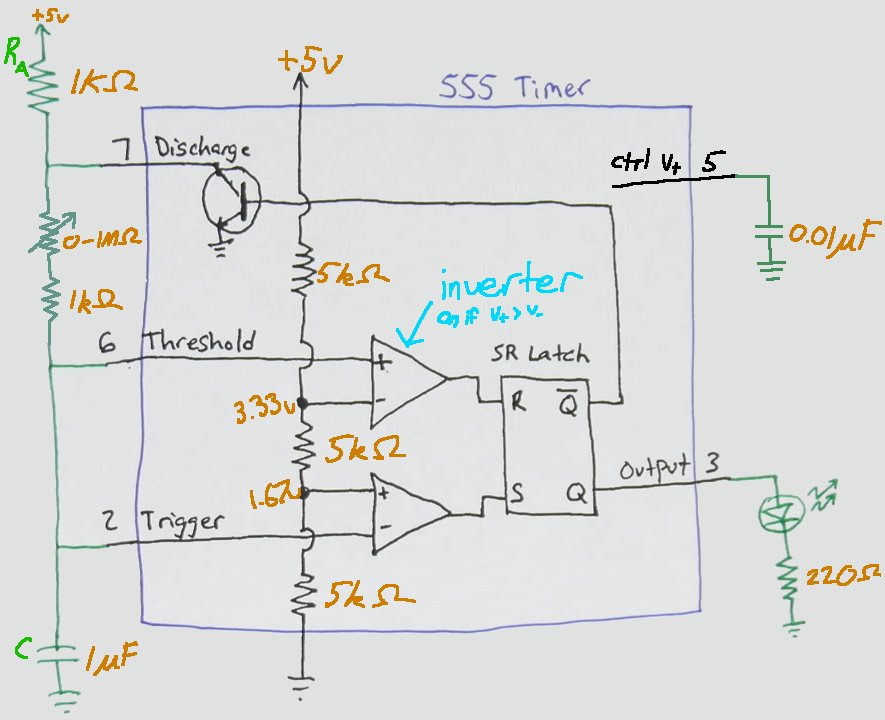
\includegraphics[width=0.8\linewidth]{../modules/clock/astable_circuit_diagram.png}
    \caption{Astable 555 Timer Circuit Diagram}
    \label{fig:astable_circuit_diagram}
  \end{center}
\end{figure}

The datasheet provides some equtions for determining the charge time (Equation \ref{eqn:astable_charge_time}), discharge time (Equation \ref{eqn:astable_discharge_time}), total period (Equation \ref{eqn:astable_period}), and frequency of oscillation (Equation \ref{eqn:astable_frequency}). \\

\begin{equation}
  \label{eqn:astable_charge_time}
  t_1 = 0.693 ( R_A + R_B ) C
\end{equation}

\begin{equation}
  \label{eqn:astable_discharge_time}
  t_2 = 0.693 ( R_B ) C
\end{equation}

\begin{equation}
  \label{eqn:astable_period}
  T = t_1 + t_2 = 0.693 ( R_A + 2 R_B ) C
\end{equation}

\begin{equation}
  \label{eqn:astable_frequency}
  f = \frac{1}{T} = \frac{1.44}{( R_A + 2 R_B ) C}
\end{equation}

\vspace{0.5cm}

The completed circuit is shown in Figure \ref{fig:astable_circuit}. Before the last few capacitors were added to the circuit, the oscilloscope probes were hooked to the positive lead of the capacitor, as well as the output of the SR latch. This data is shown in Figure \ref{fig:astable_scope}. Note: the values on both scales of the oscilloscope data are not accurate, it's the shape that's important. \\

\vspace{0.3cm}

Of particular note in Figure \ref{fig:astable_scope} is the overshoot on the output of the SR latch. This is largely caused by the impedence and inductance in the relatively long power cable, as it causes a delay in the time for the power supply to supply enough power to turn the LED on (and do the other thing that happen inside the 555 chip). This can be remedied by placing a 0.1$\mu$F capacitor across the power lines of the breadboard. Similarly, the datasheet recommends placing a 0.01$\mu$F capacitor from pin 5 to GND, to reduce noise. A plot of this data is not included as it does not show up very clearly on a cheap oscilloscope. \\

\vspace{0.3cm}

Finally, note the variable resistor (in series with a 1k$\omega$ resistor) in Figure \ref{fig:astable_circuit_diagram}, which allows the speed of the clock to be varied by controlling the flow of current into and out of the capacitor. \\

\vspace{0.3cm}

Table \ref{tab:astable_cycle} shows the operation cycle of the circuit. \\


\begin{figure}[h]
  \begin{center}
    \includegraphics[width=0.5\linewidth]{../modules/clock/astable_circuit.png}
    \caption{Astable 555 Timer Circuit}
    \label{fig:astable_circuit}
  \end{center}
\end{figure}

\begin{figure}[h]
  \begin{center}
    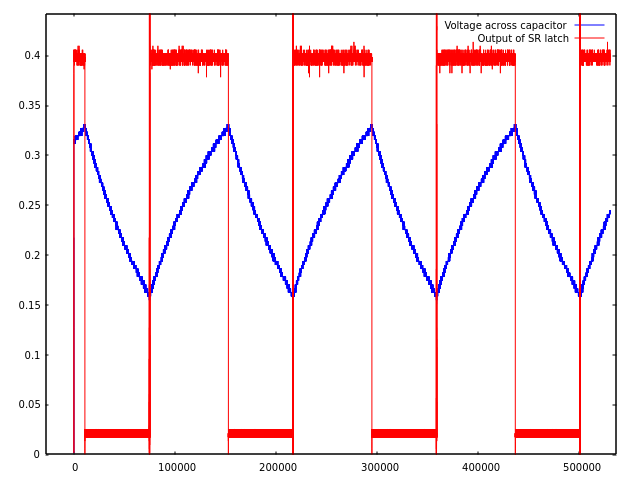
\includegraphics[width=\linewidth]{../modules/clock/astable_scope_no_caps.png}
    \caption{Astable 555 Timer Oscilloscope Data}
    \label{fig:astable_scope}
  \end{center}
\end{figure}

\begin{table}[h]
  \begin{center}
    \begin{tabular}{ c | c c c c c c c }
      Time & Circuit Status & Capacitor Voltage & S & R & Q & $\overline Q$ & Transistor \\
      \hline
      $t_0$ & Power on    & 0       & 1 & 0 & 1 & 0 & Off \\
      $t_1$ & Charging    & $>1.67$ & 0 & 0 & 1 & 0 & Off \\
      $t_2$ & Discharging & $>3.33$ & 0 & 1 & 0 & 1 & On  \\
      $t_3$ & Discharging & $<3.33$ & 0 & 0 & 0 & 1 & On  \\
      $t_4$ & Charging    & $<1.67$ & 1 & 0 & 1 & 0 & Off \\
    \end{tabular}
    \caption{Astable 555 Timer Operation Cycle}
    \label{tab:astable_cycle}
  \end{center}
\end{table}

\clearpage


\subsection{Monostable 555 Timer}
To allow us to manually advance the clock by one clock cycle, we will use a 555 timer to debounce a pushbutton. This mode of operation is referred to as monostable operation, as the circuit settles to a stable state after the capacitor is discharged.

\vspace{0.3cm}

The monostable circuit diagram is shown in Figure \ref{fig:monostable_circuit_diagram}, and the physical circuit is shown in Figure \ref{fig:monostable_circuit}. The operation cycle is shown in Table \ref{tab:monostable_cycle}, and a plot of data from the oscilloscope is shown in Figure \ref{fig:monostable_scope}.

\begin{figure}[h]
  \begin{center}
    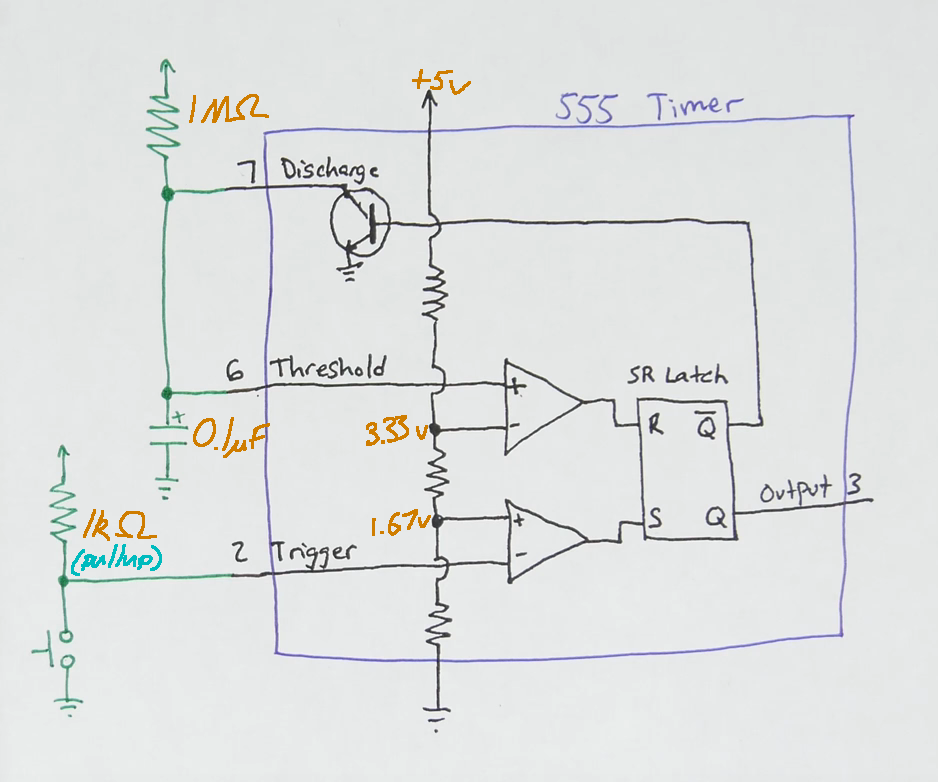
\includegraphics[width=0.8\linewidth]{../modules/clock/monostable_circuit_diagram.png}
    \caption{Monostable 555 Timer Circuit}
    \label{fig:monostable_circuit_diagram}
  \end{center}
\end{figure}

\begin{figure}[h]
  \begin{center}
    \includegraphics[width=0.7\linewidth]{../modules/clock/monostable_circuit.png}
    \caption{Monostable 555 Timer Circuit}
    \label{fig:monostable_circuit}
  \end{center}
\end{figure}

\begin{table}[ht]
  \begin{center}
    \begin{tabular}{ c | c c c c c c c }
      Time & Circuit Status & Capacitor Voltage & S & R & Q & $\overline Q$ & Transistor \\
      \hline
      $t_0$ & Power on        & 0       & 0 & 0 & x & x & x    \\
      $t_1$ & Stable          & 0       & 0 & 0 & 0 & 1 & On   \\
      $t_2$ & Button Pressed  & 0       & 1 & 0 & 1 & 0 & Off  \\
      $t_3$ & Button Released & $<3.33$ & 0 & 0 & 1 & 0 & Off  \\
      $t_4$ & Discharge       & $>3.33$ & 0 & 1 & 0 & 1 & On   \\
    \end{tabular}
    \caption{Monostable 555 Timer Operation Cycle}
    \label{tab:monostable_cycle}
  \end{center}
\end{table}

\begin{figure}[hb]
  \begin{center}
    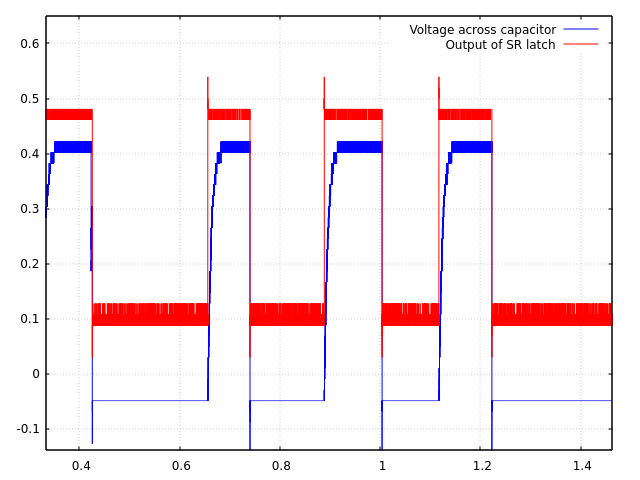
\includegraphics[width=0.9\linewidth]{../modules/clock/monostable_scope.png}
    \caption{Monostable 555 Timer Circuit}
    \label{fig:monostable_scope}
  \end{center}
\end{figure}


\subsection{Bistable 555 Timer}



\end{FlushLeft}

\clearpage

\end{document}
